\PassOptionsToPackage{unicode=true}{hyperref} % options for packages loaded elsewhere
\PassOptionsToPackage{hyphens}{url}
%
\documentclass[9pt,a4paper,]{extarticle}
\usepackage{lmodern}
\usepackage{amssymb,amsmath}
\usepackage{ifxetex,ifluatex}
\usepackage{fixltx2e} % provides \textsubscript
\ifnum 0\ifxetex 1\fi\ifluatex 1\fi=0 % if pdftex
  \usepackage[T1]{fontenc}
  \usepackage[utf8]{inputenc}
  \usepackage{textcomp} % provides euro and other symbols
\else % if luatex or xelatex
  \usepackage{unicode-math}
  \defaultfontfeatures{Ligatures=TeX,Scale=MatchLowercase}
\fi
% use upquote if available, for straight quotes in verbatim environments
\IfFileExists{upquote.sty}{\usepackage{upquote}}{}
% use microtype if available
\IfFileExists{microtype.sty}{%
\usepackage[]{microtype}
\UseMicrotypeSet[protrusion]{basicmath} % disable protrusion for tt fonts
}{}
\IfFileExists{parskip.sty}{%
\usepackage{parskip}
}{% else
\setlength{\parindent}{0pt}
\setlength{\parskip}{6pt plus 2pt minus 1pt}
}
\usepackage{hyperref}
\hypersetup{
            pdftitle={Dictionary of disease ontologies},
            pdfkeywords={disease ontologies, diseases, phenotypes, database, identifiers},
            pdfborder={0 0 0},
            breaklinks=true}
\urlstyle{same}  % don't use monospace font for urls
\usepackage[margin=1in]{geometry}
\usepackage{color}
\usepackage{fancyvrb}
\newcommand{\VerbBar}{|}
\newcommand{\VERB}{\Verb[commandchars=\\\{\}]}
\DefineVerbatimEnvironment{Highlighting}{Verbatim}{commandchars=\\\{\}}
% Add ',fontsize=\small' for more characters per line
\usepackage{framed}
\definecolor{shadecolor}{RGB}{248,248,248}
\newenvironment{Shaded}{\begin{snugshade}}{\end{snugshade}}
\newcommand{\AlertTok}[1]{\textcolor[rgb]{0.94,0.16,0.16}{#1}}
\newcommand{\AnnotationTok}[1]{\textcolor[rgb]{0.56,0.35,0.01}{\textbf{\textit{#1}}}}
\newcommand{\AttributeTok}[1]{\textcolor[rgb]{0.77,0.63,0.00}{#1}}
\newcommand{\BaseNTok}[1]{\textcolor[rgb]{0.00,0.00,0.81}{#1}}
\newcommand{\BuiltInTok}[1]{#1}
\newcommand{\CharTok}[1]{\textcolor[rgb]{0.31,0.60,0.02}{#1}}
\newcommand{\CommentTok}[1]{\textcolor[rgb]{0.56,0.35,0.01}{\textit{#1}}}
\newcommand{\CommentVarTok}[1]{\textcolor[rgb]{0.56,0.35,0.01}{\textbf{\textit{#1}}}}
\newcommand{\ConstantTok}[1]{\textcolor[rgb]{0.00,0.00,0.00}{#1}}
\newcommand{\ControlFlowTok}[1]{\textcolor[rgb]{0.13,0.29,0.53}{\textbf{#1}}}
\newcommand{\DataTypeTok}[1]{\textcolor[rgb]{0.13,0.29,0.53}{#1}}
\newcommand{\DecValTok}[1]{\textcolor[rgb]{0.00,0.00,0.81}{#1}}
\newcommand{\DocumentationTok}[1]{\textcolor[rgb]{0.56,0.35,0.01}{\textbf{\textit{#1}}}}
\newcommand{\ErrorTok}[1]{\textcolor[rgb]{0.64,0.00,0.00}{\textbf{#1}}}
\newcommand{\ExtensionTok}[1]{#1}
\newcommand{\FloatTok}[1]{\textcolor[rgb]{0.00,0.00,0.81}{#1}}
\newcommand{\FunctionTok}[1]{\textcolor[rgb]{0.00,0.00,0.00}{#1}}
\newcommand{\ImportTok}[1]{#1}
\newcommand{\InformationTok}[1]{\textcolor[rgb]{0.56,0.35,0.01}{\textbf{\textit{#1}}}}
\newcommand{\KeywordTok}[1]{\textcolor[rgb]{0.13,0.29,0.53}{\textbf{#1}}}
\newcommand{\NormalTok}[1]{#1}
\newcommand{\OperatorTok}[1]{\textcolor[rgb]{0.81,0.36,0.00}{\textbf{#1}}}
\newcommand{\OtherTok}[1]{\textcolor[rgb]{0.56,0.35,0.01}{#1}}
\newcommand{\PreprocessorTok}[1]{\textcolor[rgb]{0.56,0.35,0.01}{\textit{#1}}}
\newcommand{\RegionMarkerTok}[1]{#1}
\newcommand{\SpecialCharTok}[1]{\textcolor[rgb]{0.00,0.00,0.00}{#1}}
\newcommand{\SpecialStringTok}[1]{\textcolor[rgb]{0.31,0.60,0.02}{#1}}
\newcommand{\StringTok}[1]{\textcolor[rgb]{0.31,0.60,0.02}{#1}}
\newcommand{\VariableTok}[1]{\textcolor[rgb]{0.00,0.00,0.00}{#1}}
\newcommand{\VerbatimStringTok}[1]{\textcolor[rgb]{0.31,0.60,0.02}{#1}}
\newcommand{\WarningTok}[1]{\textcolor[rgb]{0.56,0.35,0.01}{\textbf{\textit{#1}}}}
\usepackage{longtable,booktabs}
% Fix footnotes in tables (requires footnote package)
\IfFileExists{footnote.sty}{\usepackage{footnote}\makesavenoteenv{longtable}}{}
\usepackage{graphicx,grffile}
\makeatletter
\def\maxwidth{\ifdim\Gin@nat@width>\linewidth\linewidth\else\Gin@nat@width\fi}
\def\maxheight{\ifdim\Gin@nat@height>\textheight\textheight\else\Gin@nat@height\fi}
\makeatother
% Scale images if necessary, so that they will not overflow the page
% margins by default, and it is still possible to overwrite the defaults
% using explicit options in \includegraphics[width, height, ...]{}
\setkeys{Gin}{width=\maxwidth,height=\maxheight,keepaspectratio}
\setlength{\emergencystretch}{3em}  % prevent overfull lines
\providecommand{\tightlist}{%
  \setlength{\itemsep}{0pt}\setlength{\parskip}{0pt}}
\setcounter{secnumdepth}{0}
% Redefines (sub)paragraphs to behave more like sections
\ifx\paragraph\undefined\else
\let\oldparagraph\paragraph
\renewcommand{\paragraph}[1]{\oldparagraph{#1}\mbox{}}
\fi
\ifx\subparagraph\undefined\else
\let\oldsubparagraph\subparagraph
\renewcommand{\subparagraph}[1]{\oldsubparagraph{#1}\mbox{}}
\fi

% set default figure placement to htbp
\makeatletter
\def\fps@figure{htbp}
\makeatother

\usepackage{booktabs}
\usepackage{longtable}
\usepackage{array}
\usepackage{multirow}
\usepackage{wrapfig}
\usepackage{float}
\usepackage{colortbl}
\usepackage{pdflscape}
\usepackage{threeparttable}
\usepackage[normalem]{ulem}
\usepackage{makecell}
\usepackage{xcolor}
\usepackage[]{natbib}
\bibliographystyle{plainnat}

\title{Dictionary of disease ontologies}
\author{true \and true \and true}
\date{}

\begin{document}
\maketitle
\begin{abstract}
To add
\end{abstract}

\textbf{R version}: R version 3.6.0 (2019-04-26)

\textbf{Bioconductor version}: 3.10

\textbf{Package}: 1.0.0

\hypertarget{introduction}{%
\section{Introduction}\label{introduction}}

Disease ontologies have been developed to meet the need to structure, classify, and describe diseases \citep{Gruber1993, Haendel2018, Hoehndorf2013}. As a result of the diversity in their usage a multitude of disease ontologies exist, aiming to facilitate the integration with drug information, transcriptomics and genomics information, etc. as well as to support development of novel treatments \citep{Haendel2018, Hoehndorf2013, Rappaport2013}. Disease ontologies allow a more formal description of disease; however, each often defines an independent identifier and will only link to a subset of independent biological databases \citep{Hasnain2014, Hoehndorf2013, Kibbe2015, Livingston2015, Malone2010, Rappaport2013}. While this stimulated the construction of integrated biological knowledge bases, the use of independent, ontology-specific identifiers, heterogeneous decisions on disease definitions, and the inherent presence of errors complicates integrating disease ontologies \citep{Livingston2015, Rappaport2013}. In addition, the navigation of these large integrated knowledgebase with often an inheritely complicated data model, is difficult for most, non-expert users \citep{Hasnain2014, Hu2017, Livingston2015}.

Several efforts have been made to connect the different disease ontologies themselves by generating of a single new integrative ontology \citep{Mungall2017, Shefchek2019, Rappaport2013}. Using semantic similarity the Monarch Disease Ontology (MonDO) aggregates different sources including OMIM, Orphanet, NCiT, GARD, DO, and MF \citep{Mungall2017, Shefchek2019}. Other examples is the Disease Ontology (DO) resource which aims to standardize disease descriptions and classification from a clinical perspective using equivalence mappings \citep{Cheng2013, Schriml2015, Yu2015}. The Experimental Factor Ontology (EFO) also establishes an unified ontology (not limited to diseases) by re-using several reference ontologies that lie within its scope and enriches these classess with additional axioms when needed \citep{Malone2010}. Currently, it combines information from OMIM, Orphanet, ICD9/10 and SNOMEDCT, HPO, UBERON, and MonDO \citep{EFO2019}.

Despite ongoing efforts, two issues remain to use disease ontologies efficiently: the issue of completeness and ease of access. To this end, the Dictionary of Disease Ontologies (DODO) was developed. The first issue of completeness concerns the exhaustiveness of disease cross-reference mappings \citep{Hu2017, Rappaport2013}. While efforts such as the Monarch Initiative and EFO try to integrate different disease ontologies through semantic learning and manual curation, these resources, like the different disease ontologies themselves, are currently not providing a complete mapping across different disease ontologies. By combining the information provided by the different ontologies, these cross-reference mappings can be enriched. It also allows connecting ontologies to each other that have no direct cross-reference mapping between them by indirectly inferring relationships. In addition, the existing efforts for integration are not flexible to extend easily to proprietary disease ontologies. Another challenge is the availability of an efficient and straightforward manner to access disease information through well established bioinformatics platforms (R or python) \citep{Rappaport2013, Saqi2018}. If avialble, this will facilitate a more flexible connection to the different life science resources to create a more complete disease landscape. Currently, the programmatic access provided by many ontologies often requires expertise in creating SPARQL queries and a high level of understanding of the underlying databases or data model to be able to generate more complex queries \citep{Hasnain2014, Hu2017, Rappaport2013}. The presented graph database is accompagnied by a R package that allows easy access, exploration, and definition of disease concepts of interest. It can work as the intermediate player to facilitate access and exhaustive extraction of information from other life science databases without the need to harmonize these up front. In this paper we will present DODO graphical database and R package with use cases.

\hypertarget{methods}{%
\section{Methods}\label{methods}}

\hypertarget{implementation}{%
\subsection{Implementation}\label{implementation}}

For software tool papers, this section should address how the tool works and any relevant technical details required for implementation of the tool by other developers.

In this section, an overview is presented of the DODO graphQL+ database and the accompagnying R package.

\hypertarget{data-model}{%
\subsubsection{Data model}\label{data-model}}

\begin{figure}

{\centering 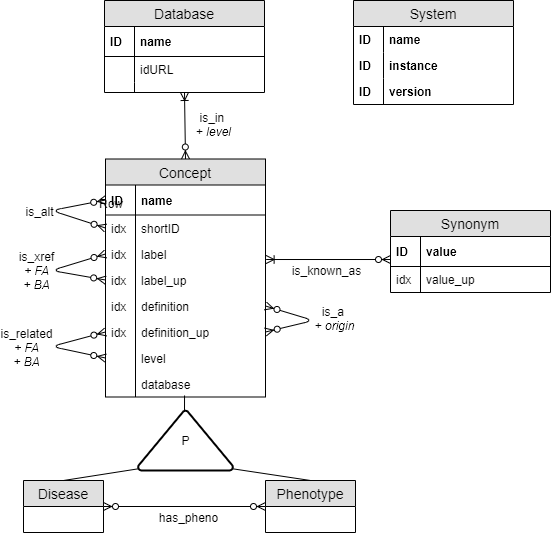
\includegraphics[width=0.5\linewidth]{/data/lfrancois/Development/DODO/inst/documentation/data-model/DODO} 

}

\caption{The DODO graph model is shown as an Entity/Relationship (ER) diagram. It consist of four types of entities (concept, disease, phenotype, database) corresponding to graph nodes. Several relationships between the nodes are described referring to graph edges. 'ID' refers to an unique entity while 'idx' indicates whether this entity is indexed.}\label{fig:dataModel}
\end{figure}

The data model underlying DODO aims to capture the relationship between disease and phenotypes as described across different databases \ref{fig:dataModel}. It relies on four types of nodes (concept, disease, phenotype, and database) each with specific proporties. A disease or phenotype nodes have the same properties with \emph{name} as their primary property. \emph{Name} is the full length identifier of a disease or phenotype, namely a concatenation of database and identifier, e.g. ``MONDO:0005027''. Additional properties are (when available) a unique (canonical) \emph{label}, disease \emph{definition}, \emph{database}, and node \emph{type}. In addition, \emph{label\_up} and \emph{definition\_up} are the uppercase version of \emph{label} and \emph{definition} respectively. Each node with class disease or phenotype is also encoded witht the class ``Concept''. Synonyms of the nodes are available through the \emph{is\_known\_as} relationship with \emph{value} and \emph{value\_up} containing the (uppercase) synonyms. A database node has only two property values, its \emph{name} (the name of the database) and url link (\emph{idURL}).

Nodes can be related to each other through different relations based on information provided by the
resources. A disease/phenotype/concept node can be related to another node belonging to a different database by the \emph{is\_xref} or \emph{is\_related} relationship. This relationship indicates nodes relating to the same or highly similar disease concepts (as defined by the original resources). The relationship is directional and has the property \emph{FA} (forward ambiguity) and \emph{BA} (backward ambiguity). As disease definitions can be implemented in a broad or narrow sense by each disease ontology, \emph{is\_xref} and \emph{is\_related} relationships across ontologies are not always unambiguous. The concept of forward and backward ambiguity is implemented to handle transitivity mapping (see below). The \emph{is\_xref} and \emph{is\_related} relationship is dependent on the direction one is traversing through and is therefore encoded twice between each node. Each of these directions has its subsequent forward and backward ambiguity information provided as properties.

Phenotype/disease/concept nodes may also be related through \emph{is\_a} directional hierarchical relationship identifying parent/child nodes based on an ontological tree. This relationship is only available between nodes of the same database with the exception of diseases defined by EFO. EFO combines the re-use of identifiers from external resources and enriches this information with additional internal disease classifiers to construct its ontology \citep{Malone2010}. To distinguish the origin of the \emph{is\_a} relationship, the property \emph{origin} is a added.

Phenotypes are highly detailed descriptions of clinical abnormalities which are used to describe disease through \emph{has\_pheno} non-directional relationship. And finally, each disease or phenotype node belongs to a database as encoded by the \emph{is\_in} relationship. This relationship is assigned the property (hierarchical) \emph{level} capturing the highest position a node has in the ontology tree.

\hypertarget{feeding-the-database}{%
\subsubsection{Feeding the database}\label{feeding-the-database}}

To construct a DODO instance, a set of script is available to load and feed a Neo4j instance. These are not exposed directly to the user instead, these scripts are available in the \emph{build/scripts} folder. The feeding of DODO is based on the parsed files of the different ontologies, a workflow on downloading and parsing for each included ontology is available through GitHub (Table \ref{tab:githubOntology}).

\begin{table}

\caption{\label{tab:githubOntology}Different disease ontologies included into DODO database and link to GitHub repository.}
\centering
\begin{tabular}[t]{ll}
\toprule
Disease ontology & GitHub\\
\midrule
Monarch Disease Ontology (MonDO) & https://github.com/Elysheba/Monarch\\
Experimental Factor Ontology (EFO) & https://github.com/Elysheba/EFO\\
Orphanet & https://github.com/Elysheba/Orphanet\\
MedGen & https://github.com/Elysheba/MedGen\\
Medical Subject Headings (MeSH) & https://github.com/Elysheba/MeSH\\
\addlinespace
Human Phenotype Ontology (HPO) & https://github.com/patzaw/HPO\\
ClinVar & https://github.com/patzaw/ClinVar\\
Disease Ontology (DO) & https://github.com/Elysheba/DO\\
International Classification of Diseases (ICD11) & https://github.com/Elysheba/ICD11\\
\bottomrule
\end{tabular}
\end{table}

The different steps are briefly described below:

\begin{enumerate}
\def\labelenumi{\arabic{enumi}.}
\item
  Creating the relationship tables based on the information from the different resources
\item
  Creating a new DODO instance and importing the relationship tables
\item
  Compiling the instance into a Dgraph image
\item
  Start the new instance
\end{enumerate}

\hypertarget{availability}{%
\subsubsection{Availability}\label{availability}}

The DODO instance build using the workflow described above is provided as a Docker image \citep{Docker2017} here.
This instance is build on information from the following disease ontologies listed in (Table \ref{tab:githubOntology}.

\hypertarget{s3-object}{%
\subsubsection{S3 object}\label{s3-object}}

The center object used through the DODO R package is the disease network or disNet S3 object. It captures all information (disease node information, hierarchical information, phenotype information, and cross-reference informatino) around a disease and is structured as shown in Table \ref{tab:disNetObject}

\begin{table}

\caption{\label{tab:disNetObject}The center object used through the DODO R package is the disease network or disNet S3 object. It captures all information (disease node information, hierarchical information, phenotype information, and cross-reference informatino) around a disease.}
\centering
\resizebox{\linewidth}{!}{
\begin{tabular}[t]{ll}
\toprule
Part & Content\\
\midrule
\rowcolor{gray!6}  \addlinespace[0.3em]
\multicolumn{2}{l}{\textbf{nodes}}\\
\hspace{1em}id & disease ids (database:shortID)\\
\hspace{1em}database & disease databases\\
\rowcolor{gray!6}  \hspace{1em}shortID & disease short identifiers\\
\hspace{1em}label & disease labels\\
\rowcolor{gray!6}  \hspace{1em}definition & disease descriptions\\
\hspace{1em}level & maximum level the identifier holds in the hierarchical ontology tree\\
\rowcolor{gray!6}  \hspace{1em}type & type of node (disease or phenotype)\\
\addlinespace[0.3em]
\multicolumn{2}{l}{\textbf{synonyms}}\\
\hspace{1em}id & disease ids\\
\rowcolor{gray!6}  \hspace{1em}synonym & disease synonyms\\
\addlinespace[0.3em]
\multicolumn{2}{l}{\textbf{children}}\\
\hspace{1em}parent & parent disease ids\\
\rowcolor{gray!6}  \hspace{1em}child & child disease ids\\
\hspace{1em}origin & ontology of origin where the parent/child relationship is recorded\\
\rowcolor{gray!6}  \addlinespace[0.3em]
\multicolumn{2}{l}{\textbf{xref}}\\
\hspace{1em}from & disease 1 ids\\
\hspace{1em}to & disease 2 ids\\
\rowcolor{gray!6}  \hspace{1em}ur & unique cross-reference identifier\\
\hspace{1em}forwardAmbiguity & number of cross-references between disease 1 and database 2\\
\rowcolor{gray!6}  \hspace{1em}backwardAmbiguity & number of cross-references between disease 2 and database 1\\
\addlinespace[0.3em]
\multicolumn{2}{l}{\textbf{alt}}\\
\hspace{1em}type & type of cross-reference edge (is\_xref or is\_related)\\
\rowcolor{gray!6}  \hspace{1em}id & current identifier\\
\addlinespace[0.3em]
\multicolumn{2}{l}{\textbf{pheno}}\\
\hspace{1em}alt & deprecated identifier\\
\rowcolor{gray!6}  \hspace{1em}disease & disease identifier\\
\addlinespace[0.3em]
\multicolumn{2}{l}{\textbf{seed}}\\
\hspace{1em}phenotype & phenotype identifier\\
\rowcolor{gray!6}  seed & vector of disease ids used to seed the disNet\\
\bottomrule
\end{tabular}}
\end{table}

In addition, a \emph{setDisNet} S3 object is also available which consists of a list of \emph{disNet} objects. Figure @ref\{fig:disNet\} shows an example disNet object for epilepsy.

\hypertarget{operation}{%
\subsection{Operation}\label{operation}}

The data model is implemented using the Neo4j graph database which using the Cypher query language \citep{Neo4j2020}. One accompagnying R package \emph{DODO} was developed to connect and query the resource. It provides higher level functions to query the Neo4j graph database based on the described data model (above) \citep{R2019}.

The minimal system requirements are:

\begin{itemize}
\item
  R \(\geq\) 3.6
\item
  Operating system: Linux, macOS, Windows
\item
  Memory \(\geq\) 4GB RAM
\end{itemize}

The graph database has been implemented with Neo4j 3.4.9 \citep{Neo4j2020}, the DODO R package uses the following packages:

\begin{itemize}
\item
  \emph{\href{https://CRAN.R-project.org/package=dplyr}{dplyr}} \citep{Wickham2019}
\item
  \emph{\href{https://CRAN.R-project.org/package=tibble}{tibble}} \citep{Muller2019}
\item
  \emph{\href{https://CRAN.R-project.org/package=neo2R}{neo2R}} \citep{Godard2020}
\item
  \emph{\href{https://CRAN.R-project.org/package=rlist}{rlist}} \citep{Ren2016}
\item
  \emph{\href{https://CRAN.R-project.org/package=stringr}{stringr}} \citep{Wickham2019b}
\item
  \emph{\href{https://CRAN.R-project.org/package=readr}{readr}} \citep{Wickham2018}
\item
  \emph{\href{https://CRAN.R-project.org/package=visNetwork}{visNetwork}} \citep{Almende2017}
\item
  \emph{\href{https://CRAN.R-project.org/package=shinythemes}{shinythemes}} \citep{Chang2018}
\item
  \emph{\href{https://CRAN.R-project.org/package=DT}{DT}} \citep{Xie2019}
\item
  \emph{\href{https://CRAN.R-project.org/package=igraph}{igraph}} \citep{Csardi2006}
\item
  \emph{\href{https://CRAN.R-project.org/package=shiny}{shiny}} \citep{Chang2019}
\item
  \emph{\href{https://CRAN.R-project.org/package=BiocStyle}{BiocStyle}}\citep{Oles2020}
\end{itemize}

\hypertarget{querying-the-database}{%
\subsubsection{Querying the database}\label{querying-the-database}}

The DODO R package combines several functions to construct, interact, and explore such a disNet object. These will be briefly outlined in the sections below. These functions also split or cluster a disNet, generating a list of disNet object, captured by the S3 object setDisNet.

DODO R package provides function to allow four different scopes: building and interacting with a disNet of setDisNet object, visualizing a disNet, converting disease and phenotype concepts to different ontologies, and several utility functions to connect to DODO graph database or obtain low level information on identifiers. The Table \ref{tab:functions} briefly list all function available within the package, as well as a short description and identification of the scope.

\begin{table}

\caption{\label{tab:functions}Summary of the available functions in DODO with a short description and identification of their scope.}
\centering
\resizebox{\linewidth}{!}{
\begin{tabular}[t]{lll}
\toprule
Function & Description & scope\\
\midrule
\rowcolor{gray!6}  build\_disNet & Building a network of disease identifiers & Build and interact\\
extend\_disNet & Extending a disNet by different edges & Build and interact\\
\rowcolor{gray!6}  filter\_by\_id & Filtering a disNet by id & Build and interact\\
filter\_by\_database & Filtering a disNet by database & Build and interact\\
\rowcolor{gray!6}  focus\_disNet & Focus on identifiers of interest and its neighbors & Build and interact\\
\addlinespace
cluster\_disNet & Clustering a disNet, generates a setDisNet & Build and interact\\
\rowcolor{gray!6}  setdiff\_disNet & Substract one disNet from another & Build and interact\\
split\_disNet & Split a disNet based on a list of identifiers into a setDisNet & Build and interact\\
\rowcolor{gray!6}  explore\_disNet & Visualizes a datatable to explore a disNet & Visualize\\
show\_relations & Visualizes cross-reference relationships for the provided identifier & Visualize\\
\addlinespace
\rowcolor{gray!6}  plot.disNet & Visualizes a disNet using visNetwork & Visualize\\
convert\_concept & Convert the provided set of identifiers to another ontology or between concepts & Conversion\\
\rowcolor{gray!6}  get\_related & Convert function for ontologies separated by *is\_related* edges mainly & Conversion\\
check\_dodo\_connection & Check connection with DODO graphical database & Utility\\
\rowcolor{gray!6}  connect\_to\_dodo & Establish connection with DODO graphical database & Utility\\
\addlinespace
forget\_dodo\_connection & Forget a saved connection to DODO & Utility\\
\rowcolor{gray!6}  list\_dodo\_connections & List all saved connections to DODO & Utility\\
call\_dodo & Calls a function on the DODO graphical database & Utility\\
\rowcolor{gray!6}  show\_dodo\_model & Return DODO data model & Utility\\
get\_version & Return DODO database version & Utility\\
\addlinespace
\rowcolor{gray!6}  get\_concept\_url & Returns concept url & Utility\\
list\_database & Lists databases in DODO & Utility\\
\rowcolor{gray!6}  list\_node\_type & Lists node type in DODO & Utility\\
get\_ontology & Returns whole ontology & Utility\\
\rowcolor{gray!6}  describe\_concept & Returns concept description & Utility\\
\bottomrule
\end{tabular}}
\end{table}

\hypertarget{transitivity-mapping}{%
\subsubsection{Transitivity mapping}\label{transitivity-mapping}}

As a consequence of the different way ontologies define disease (or phenotype) concepts, some cross-reference edges connect identifiers that are not exactly equal. Therefore, some cross-reference edges are trusted more than others. Ontologies such as MONDO or EFO use more narrow disease definitions than others like ICD10 or ICD9. If cross-reference edges are all considered equal without taking this distinction into account, it will result in the return of more distantly related concepts when traversing these edges. Table \ref{tab:exampleAmb} shows an example of ``Coffin-Lowry'' syndrome (Orphanet identifier ``192'') for which most cross-reference identifiers are defined similarly. However, its cross-reference to ICD10 deals with a very broad term of ``Conginetal malformation syndromes predominantly affecting facial appearance'' (``ICD:Q87.0''). This identifier is highly ambiguous and has 284 different direct cross-referenced disease identifiers.

\begin{table}

\caption{\label{tab:exampleAmb}The EFO (and Orphanet) identifier for Coffin-Lowry syndrome (ORPHA:192) is cross-referenced to 21 different identifiers. Many of these cross-references are more or less equivalent to the original identifier (disease labels are only available when present in the parsed resources. Otherwise only a disease identifier is available). However, among its cross-references it also links to an ICD10 identifier (Q87.0) which is a broad term of 'Congenital malformation syndromes predominantly affecting facial appearance'. This identifier is highly ambiguous and links directly to 284 disease concepts.}
\centering
\resizebox{\linewidth}{!}{
\begin{tabular}[t]{ll}
\toprule
Disease identifier & Disease label\\
\midrule
\rowcolor{gray!6}  MedGen:C0795900 & Coffin syndrome 1\\
ORPHA:192 & Coffin-Lowry syndrome\\
\rowcolor{gray!6}  MONDO:0010561 & Coffin-Lowry syndrome\\
ClinVar:823 & Coffin-Lowry syndrome\\
\rowcolor{gray!6}  MedGen:C0265252 & Coffin-Lowry syndrome\\
\addlinespace
DOID:3783 & Coffin-Lowry syndrome\\
\rowcolor{gray!6}  UMLS:C0265252 & Coffin-Lowry syndrome\\
MeSH:D038921 & Coffin-Lowry Syndrome\\
\rowcolor{gray!6}  OMIM:303600 & COFFIN-LOWRY SYNDROME\\
ICD10:Q87.0 & Congenital malformation syndromes predominantly affecting facial appearance\\
\addlinespace
\rowcolor{gray!6}  MeSH:C536435 & NA\\
SNOMEDCT:15182000 & NA\\
\rowcolor{gray!6}  OMIM:300075 & NA\\
UMLS:C0795900 & NA\\
\rowcolor{gray!6}  GTR:GTRT000007048 & NA\\
\addlinespace
ICD9:759.89 & NA\\
\rowcolor{gray!6}  OMIM:300075.0011 & NA\\
GTR:GTRT000000823 & NA\\
\rowcolor{gray!6}  NCIt:C84643 & NA\\
GARD:6123 & NA\\
\addlinespace
\rowcolor{gray!6}  GARD:0008589 & NA\\
SNOMEDCT\_US\_2019\_09\_01:15182000 & NA\\
\rowcolor{gray!6}  GARD:0006123 & NA\\
\bottomrule
\end{tabular}}
\end{table}

The concept of \emph{ambiguity} is introduced to identify nodes that have many cross-references to the same database. Cross-reference edges are implemented in a directional manner in Neo4j, therefore both a forward (FA) and backward (BA) ambiguity is calculated and encoded on every direction. As it is often desired to move from a broader concept to a more narrow one, no filtering on forward ambiguity is put in place. However, the opposite, namely moving from a more narrow and through a broader concept is not always desired. This can result in an exponential increase of converted/expanded identifiers that are only distantly related to the original identifier.

In addition to the concept of \emph{ambiguity}, two types of cross-reference edges encoded in DODO: \emph{is\_xref} and \emph{is\_related}. The \emph{is\_xref} edge is used for equal cross-reference relationships where the concepts relate more directly to each other (similar concept definitions). The \emph{is\_related} edge is used for all other cross-reference edges. These edges are based on the sum of forward and backward ambiguities between databases to quantify the symmetry between them and knowledge of how ontologies deal with disease concepts. Ontologies included for this quantification are: MoNDO, EFO, Orphanet, Orphanet, OMIM, MedGen, UMLS, MeSH, ICD10, ICD9, DOID, ClinVar, MEDDRA, GARD, SNOMEDct, and NCIt. The heatmap (Figure \ref{fig:heatmapAmbiguity}) shows the \(log_{10}\) transformed maximum total ambiguity between ontologies.

\begin{figure}

{\centering 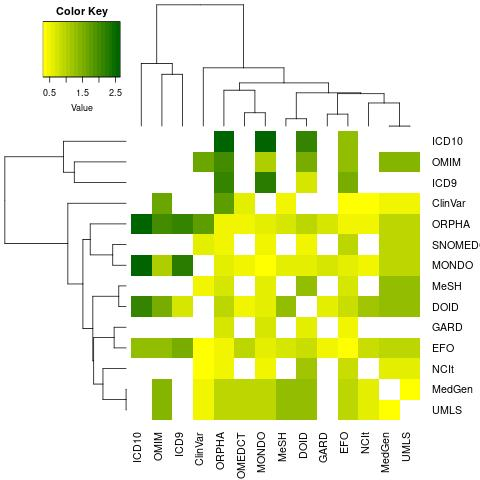
\includegraphics[width=0.5\linewidth]{/data/lfrancois/Development/DODO/inst/documentation/DODO-F1000-publication/fig/heatmap_ambiguity} 

}

\caption{The heatmap shows the maximum value of total ambiguity between ontologies using a $log_{10}$ transformation. While many ontologies are using concepts of similar level as identified by low total ambiguity, a few can be identified that are more ambiguous in their mappings. The 'optimal' ambiguity for a *is\_xref* edges is determinged by comparing the number of conversions when incrementally increasing the cutoff of total ambiguity to defining a cross-reference edge between ontologie of either *is\_xref* or *is\_related* and knowledge of the way disease concepts are defined within ontologies.}\label{fig:heatmapAmbiguity}
\end{figure}

Figure \ref{fig:boxplotAmbiguity} shows the number of conversions per identifier for MonDO when incrementally increasing the cutoff for the (total) ambiguity to define ontologies connected through \emph{is\_xref} and \emph{is\_related} edges. A very low cutoff would not return all cross-reference identifiers while a too high cutoff impact especially a few identifiers strongly with the return of many, lesser related, cross-reference identifiers.

\begin{figure}

{\centering 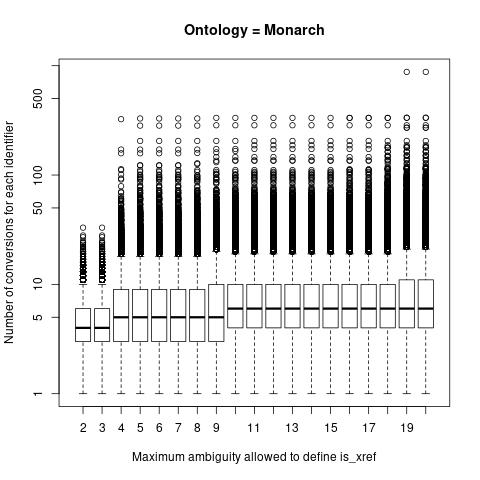
\includegraphics[width=0.5\linewidth]{/data/lfrancois/Development/DODO/inst/documentation/DODO-F1000-publication/fig/boxplot_ambiguity_conversion_mondo} 

}

\caption{Number of conversions comparing incremental cutoffs in the (total) ambiguity to define *is\_xref* and *is\_related* cross-reference edges on an ontology scale (example of MonDO ontology).}\label{fig:boxplotAmbiguity}
\end{figure}

By comparing the results and relationship between the different ontologies with a (total) ambiguity equal or lower than four are considered as \emph{is\_xref}. An exception is used for ICD10 and ICD9 which are never connected through an \emph{is\_xref} edge except between themselves. An additional exception is put in place for OMIM and Orphanet, which often define very narrow subtypes of diseases and therefore will be still encoded as an \emph{is\_xref} edge.

\hypertarget{results}{%
\section{Results}\label{results}}

The table below shows the number of nodes available through each disease ontology, in total there are 586468 nodes (Figure @ref\{fig:listDB)) in this DODO instance.

\begin{figure}

{\centering 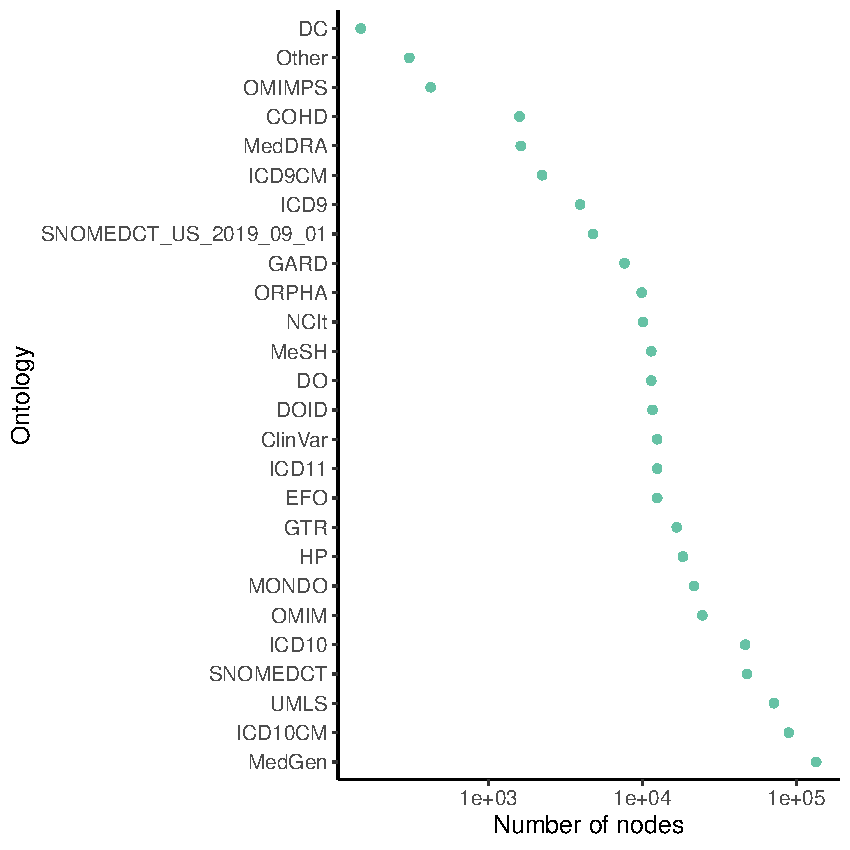
\includegraphics[width=0.5\linewidth,height=0.5\textheight]{DODO-F1000-publication_files/figure-latex/listDB-1} 

}

\caption{Overview of the number of nodes present for each disease ontology in DODO.}\label{fig:listDB}
\end{figure}

\hypertarget{use-cases}{%
\section{Use cases}\label{use-cases}}

\hypertarget{converting-concepts}{%
\subsection{Converting concepts}\label{converting-concepts}}

One of the basic functionalities of DODO is the ability to convert disease and phenotype identifiers. The conversion of identifiers generally performed in two steps based on the type of cross-reference edges and ambiguity values. Four separate use cases can be identified based on the parameters for converting within the same concept, e.g.~converting one disease identifier to other disease ontologies.

A first and default conversion consists of two steps, a first using the transitivity of \emph{is\_xref} edges followed by an addition step using both types of cross-reference edges to obtain the indirect cross-references (parameters ``step = NULL'' and ``intranstivity\_ambiguity = NULL''). The default conversion can be used to get all identifiers around a disease concept whether broad or narrowly related or when converting from a more narrow concept to a broader concept. In general when the aim is to reach a broader concept related to the original identifiers but not move through it, it is recommended to put not filter on the \emph{intransitive\_ambiguity}. For transitivity mapping using \emph{is\_xref} edges only it is strongly recommended to use the default filtering on ambiguity by limiting (backward) ambiguity to one. The second step is a intransitive mapping where both \emph{is\_related} and \emph{is\_xref} cross-reference edges are traversed with one step to get the direct cross-reference identifiers. In Figure \ref{fig:extension} an example is presented of the extension starting from the MonDO identifier ``MONDO:0005027'' encoding ``Epilepsy''. The transitive mapping with filtering on ambiguity moves between the \emph{is\_xref} mapping only in which a higher trust is placed. The final intransitive mapping step will return all nodes related through either an \emph{is\_related} or \emph{is\_xref} edge with no filtering as all ambigious relations want to be returned but not used when extending.

\begin{figure}

{\centering 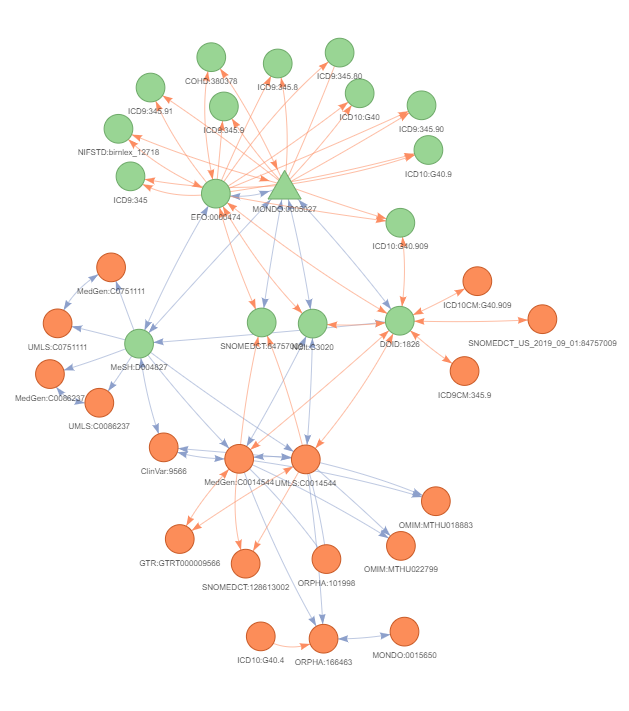
\includegraphics[width=8.42in]{/data/lfrancois/Development/DODO/inst/documentation/DODO-F1000-publication/fig/disNetExtension} 

}

\caption{A disNet constructed and subsequently extended using only cross-reference relations using the MonDO identifier for 'Epilepsy' ('MONDO:0005027') as an example. This extension is performed in two phases. First, the transitive mapping uses the *is\_xref* edges (blue edges) wich are trusted to a larger extend to obtain all relations with filtering on ambiguity (backward ambiguity = 1) (green nodes). The second steps uses no filtering as all relations (ambiguous or not) need to be returned but not used while extending (red nodes). This final intransitive mapping step will return all nodes related through either an *is\_related* (orange edges) or *is\_xref* edge with no filtering as all.}\label{fig:extension}
\end{figure}

A second case is the return of direct cross-references only without the use of transitivty to return indirect relations (parameter ``step = 1''). For the same identifier ``MONDO:0005027'', Table @ref\{tab:step1\} shows only the direct cross-references.

\begin{table}

\caption{\label{tab:step1}Conversion of 'MONDO:0005027' (epilepsy) returning only direct cross-references using parameters 'step = 1'}
\centering
\resizebox{\linewidth}{!}{
\begin{tabular}[t]{lll}
\toprule
from & to & label\\
\midrule
\rowcolor{gray!6}  MONDO:0005027 & MONDO:0005027 & epilepsy\\
MONDO:0005027 & ICD9:345.8 & epilepsy\\
\rowcolor{gray!6}  MONDO:0005027 & COHD:380378 & Epilepsy\\
MONDO:0005027 & ICD9:345.90 & Epilepsy, unspecified, not intractable, without status epilepticus\\
\rowcolor{gray!6}  MONDO:0005027 & ICD10:G40.9 & NA\\
\addlinespace
MONDO:0005027 & ICD9:345.9 & NA\\
\rowcolor{gray!6}  MONDO:0005027 & NIFSTD:birnlex\_12718 & NA\\
MONDO:0005027 & ICD9:345.80 & NA\\
\rowcolor{gray!6}  MONDO:0005027 & ICD9:345 & NA\\
MONDO:0005027 & ICD10:G40.909 & NA\\
\addlinespace
\rowcolor{gray!6}  MONDO:0005027 & ICD9:345.91 & NA\\
MONDO:0005027 & ICD10:G40 & epilepsy\\
\rowcolor{gray!6}  MONDO:0005027 & SNOMEDCT:84757009 & NA\\
MONDO:0005027 & DOID:1826 & NA\\
\rowcolor{gray!6}  MONDO:0005027 & MeSH:D004827 & Epilepsy and recurrent seizures\\
\addlinespace
MONDO:0005027 & NCIt:C3020 & Epilepsy, unspecified\\
\rowcolor{gray!6}  MONDO:0005027 & EFO:0000474 & NA\\
\bottomrule
\end{tabular}}
\end{table}

A third use case can be used to focus on concepts that are equivalent to each other and not return more broadly defined concepts. This can be a good practise when converting between ontologies that define concept similarly. With parameters `step = NULL' and `intransitive\_ambiguity = 1' disease identifiers are convert using transitivitity to return indirect mappings while using an additional filter on ambiguity for the final intransitive step.

\begin{table}

\caption{\label{tab:unnamed-chunk-3}Conversion of 'MONDO:0005027' (epilepsy) using transtivity mapping but only returning equivalent concepts in the final step by filtering on intransitive\_ambiguity}
\centering
\resizebox{\linewidth}{!}{
\begin{tabular}[t]{lll}
\toprule
from & to & label\\
\midrule
\rowcolor{gray!6}  MONDO:0005027 & MONDO:0005027 & epilepsy syndrome\\
MONDO:0005027 & ICD10:G40 & Epilepsy, unspecified, not intractable, without status epilepticus\\
\rowcolor{gray!6}  MONDO:0005027 & ICD9:345 & Epilepsy syndrome\\
MONDO:0005027 & ICD10:G40.909 & epilepsy\\
\rowcolor{gray!6}  MONDO:0005027 & ICD9:345.91 & epilepsy\\
\addlinespace
MONDO:0005027 & NIFSTD:birnlex\_12718 & Epilepsy\\
\rowcolor{gray!6}  MONDO:0005027 & ICD9:345.9 & Epilepsy, Cryptogenic\\
MONDO:0005027 & ICD9:345.8 & Epilepsy\\
\rowcolor{gray!6}  MONDO:0005027 & COHD:380378 & Awakening Epilepsy\\
MONDO:0005027 & ICD9:345.90 & Epilepsy\\
\addlinespace
\rowcolor{gray!6}  MONDO:0005027 & ICD10:G40.9 & Epilepsy, unspecified, not intractable, without status epilepticus\\
MONDO:0005027 & EFO:0000474 & NA\\
\rowcolor{gray!6}  MONDO:0005027 & SNOMEDCT:84757009 & NA\\
MONDO:0005027 & DOID:1826 & NA\\
\rowcolor{gray!6}  MONDO:0005027 & MeSH:D004827 & Epilepsy\\
\addlinespace
MONDO:0005027 & NCIt:C3020 & NA\\
\rowcolor{gray!6}  MONDO:0005027 & MedGen:C0014544 & NA\\
MONDO:0005027 & UMLS:C0014544 & NA\\
\rowcolor{gray!6}  MONDO:0005027 & ClinVar:9566 & NA\\
MONDO:0005027 & MedGen:C0086237 & NA\\
\addlinespace
\rowcolor{gray!6}  MONDO:0005027 & UMLS:C0086237 & NA\\
MONDO:0005027 & MedGen:C0751111 & epilepsy\\
\rowcolor{gray!6}  MONDO:0005027 & UMLS:C0751111 & NA\\
MONDO:0005027 & ICD10CM:G40.909 & NA\\
\rowcolor{gray!6}  MONDO:0005027 & ICD9CM:345.9 & Epilepsy and recurrent seizures\\
\addlinespace
MONDO:0005027 & SNOMEDCT\_US\_2019\_09\_01:84757009 & Epilepsy, unspecified\\
\rowcolor{gray!6}  MONDO:0005027 & ICD9:345.80 & NA\\
MONDO:0005027 & GTR:GTRT000009566 & NA\\
\rowcolor{gray!6}  MONDO:0005027 & SNOMEDCT:128613002 & NA\\
MONDO:0005027 & OMIM:MTHU018883 & NA\\
\addlinespace
\rowcolor{gray!6}  MONDO:0005027 & ORPHA:166463 & NA\\
MONDO:0005027 & OMIM:MTHU022799 & NA\\
\rowcolor{gray!6}  MONDO:0005027 & MONDO:0015650 & NA\\
\bottomrule
\end{tabular}}
\end{table}

Finally, a specific conversion procedure is recommended for the ontologies that consider disease concepts that are less connected through \emph{is\_xref} edges to the ``core'' ontologies in DODO (e.g.~MonDO, EFO, MedGen, etc.). Ontologies of ICD10, ICD9, ClinVar frequently report only those ontologies that are mapped using \emph{is\_related} cross-reference edges. When converting from these identifiers as a starting point, the conversion will not be able to return cross-reference relationship to all other database (even when they are avialable, Figure \ref{fig:icd10Convert}). It limits or removes the effect of the transitive mapping. Therefore, for these ontologies it is recommend that in addition to the standard conversion, an additional step of intransitive mapping is performed afterwards which is implemented in the function \emph{get\_related} (Figure \ref{fig:getRelated}).

\begin{figure}

{\centering 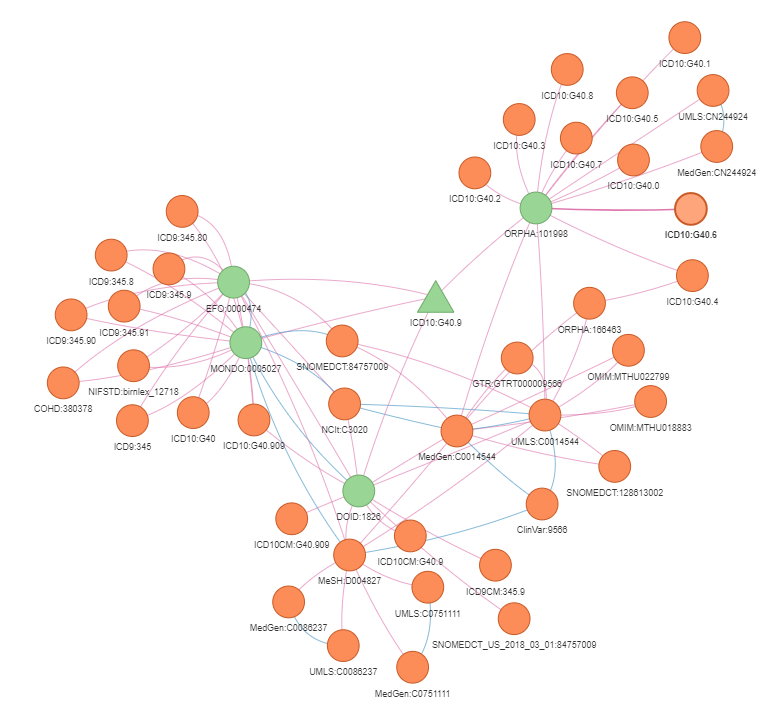
\includegraphics[width=1\linewidth]{/data/lfrancois/Development/DODO/inst/documentation/DODO-F1000-publication/fig/get_related_ambiguity_NULL_G409} 

}

\caption{Comparison of the default conversion results with the output of the specific conversion for ontologies with limited connections through is\_xref edges (blue edges). The example is the ICD10 identifier G40.9 (Epilepsy). The nodes in green signify those return through both methods, while the nodes in orange are only returned using the more specific approach for this type of ontology. In addition, the edges in blue represent is\_xref edges, while those in pink present is\_related edges between nodes (with no specification for ambiguity for simplicity).}\label{fig:getRelated}
\end{figure}

Conversion can also be used to convert between concept, i.e.~from disease identifier to phenotype identifiers or vice versa. This conversion is handled in two distinct phases. First, depending on the options listed above, identifiers are converted within the same concept. When this is not required, using parameter ``step = NA'' the conversion within the same concept can be avoided. The second phase converts between concepts by returning phenotype or disease nodes directly related to the original identifiers (including the converted identifiers obtain in the first phase).

\hypertarget{building-a-disnet}{%
\subsection{Building a disNet}\label{building-a-disnet}}

Another core concept in DODO is the S3 \emph{disNet} object which contains all information on diseases/phenotypes and their internal relationships. This object can be constructed using helper functions starting from disease identifiers or search terms (\emph{build\_disnet}).

\begin{Shaded}
\begin{Highlighting}[]
\NormalTok{disNet <-}\StringTok{ }\KeywordTok{build_disNet}\NormalTok{(}\DataTypeTok{id =} \KeywordTok{c}\NormalTok{(}\StringTok{"MONDO:0005144"}\NormalTok{))}

\NormalTok{disNet <-}\StringTok{ }\KeywordTok{build_disNet}\NormalTok{(}\DataTypeTok{term =} \StringTok{"amyotrophic lateral sclerosis"}\NormalTok{, }
                       \DataTypeTok{fields =} \KeywordTok{c}\NormalTok{(}\StringTok{"label"}\NormalTok{, }\StringTok{"synonym"}\NormalTok{))}
\end{Highlighting}
\end{Shaded}

\hypertarget{extending-a-disnet}{%
\subsection{Extending a disNet}\label{extending-a-disnet}}

When building a \emph{disNet} by either identifier(s) or search term(s), the resulting \emph{disNet} will likely not contain the complete information on that particular disease landscape. The \emph{extend\_disNet} function enriches the disNet to include addition cross-reference identifiers, child/parent terms, annotated phenotypes/disease, or alternative identifieres when available. In concordance with the conversion procedure, extension follows the same two-step approach. Please refer to paragraph @ref(Converting concepts) for more details and the different use cases.

Of specific note is the extension to (or from) phenotype information. Within one extension all different parameters (xref, child, parent, alt, and disease/phenotype) can be supplied with the exception that it is not possible to extend to both disease and phenotype simultaneously. Extending to or from phenotypes does not employ the transitivity mechanism but is performed as a final step (similar to conversion, please refer to paragraph @ref\{Converting concepts\} for more details).

\begin{Shaded}
\begin{Highlighting}[]
\NormalTok{disNet <-}\StringTok{ }\KeywordTok{build_disNet}\NormalTok{(}\DataTypeTok{id =} \KeywordTok{c}\NormalTok{(}\StringTok{"HP:0003394"}\NormalTok{, }\StringTok{"HP:0002180"}\NormalTok{, }\StringTok{"HP:0002878"}\NormalTok{))}
\NormalTok{disNet <-}\StringTok{ }\KeywordTok{extend_disNet}\NormalTok{(}\DataTypeTok{disNet =}\NormalTok{ disNet, }\DataTypeTok{relations =} \StringTok{"disease"}\NormalTok{)}
\NormalTok{disNet}
\end{Highlighting}
\end{Shaded}

\begin{verbatim}
## # A tibble: 397 x 7
##    id      label            definition            shortID level type    database
##    <chr>   <chr>            <chr>                 <chr>   <int> <chr>   <chr>   
##  1 MONDO:~ glycogen storag~ "Phosphoglycerate ki~ 0010392    11 Concep~ MONDO   
##  2 OMIM:6~ NEURODEGENERATI~ "NEURODEGENERATION W~ 610217     NA Concep~ OMIM    
##  3 MONDO:~ adult-onset dis~ "Adult-onset distal ~ 0018006    10 Concep~ MONDO   
##  4 MONDO:~ Charcot-Marie-T~ "Autosomal dominant ~ 0011675     9 Concep~ MONDO   
##  5 OMIM:6~ MOTOR NEURON DI~ "MOTOR NEURON DISEAS~ 600333     NA Concep~ OMIM    
##  6 MONDO:~ pure mitochondr~ "Pure mitochondrial ~ 0016807    11 Concep~ MONDO   
##  7 ORPHA:~ Congenital musc~ "Congenital muscular~ 258         8 Concep~ ORPHA   
##  8 OMIM:3~ MITOCHONDRIAL C~ "MITOCHONDRIAL COMPL~ 301021     NA Concep~ OMIM    
##  9 ORPHA:~ Nocardiosis      "Nocardiosis is a lo~ 31204       4 Concep~ ORPHA   
## 10 ORPHA:~ Mitochondrial e~ " mutation is charac~ 1194        9 Concep~ ORPHA   
## # ... with 387 more rows
## 
## The disNet contains:
##  -  394 disease nodes from 6 ontologies and 3 phenotype nodes from 1 ontologies 
##  -  2206 synonyms of the disease nodes
##  -  0 parent/child edges
##  -  0 crossreference edges
##  -  0 alternative edges
##  -  398 phenotype edges
##  -  The disNet was build based on 3 seeds
\end{verbatim}

\hypertarget{reviewing}{%
\subsection{Reviewing}\label{reviewing}}

Often after extending it is necessary to review the returned \emph{disNet} to assess whether all nodes are of interest. This process can be simplified by considering clusters of cross-references (nodes dealing with similar concepts) using the \emph{cluster\_disNet} functionality. Instead of reviewing each nodes, the different clusters can be reviewed to identify those of interest while using the relationships between nodes to address equivalent nodes simultaneously (Table \ref{tab:cldisNet}).

\begin{table}

\caption{\label{tab:cldisNet}Annotation of the different cross-reference clusters of nodes identified for a disNet around 'amyotrophic lateral sclerosis'. The annotation is obtained from node within the cluster with the highest order in its disease ontology ('level') and avialability of label information.}
\centering
\resizebox{\linewidth}{!}{
\begin{tabular}[t]{rrlrl}
\toprule
cluster & clusterSize & id & level & values\\
\midrule
\rowcolor{gray!6}  1 & 150 & ICD10CM:G12.21 & 4 & Amyotrophic lateral sclerosis\\
2 & 22 & MONDO:0017161 & 7 & frontotemporal dementia with motor neuron disease\\
\rowcolor{gray!6}  3 & 2 & MedGen:C1862940 & NA & Amyotrophic Lateral Sclerosis, Autosomal Recessive\\
4 & 9 & ORPHA:357043 & 6 & Amyotrophic lateral sclerosis type 4\\
\rowcolor{gray!6}  5 & 3 & MedGen:C3542025 & NA & Amyotrophic lateral sclerosis 1, autosomal recessive\\
\addlinespace
6 & 8 & MONDO:0005145 & 8 & sporadic amyotrophic lateral sclerosis\\
\rowcolor{gray!6}  7 & 6 & MONDO:0014640 & 10 & FTDALS3\\
8 & 5 & MONDO:0008781 & 10 & juvenile amyotrophic lateral sclerosis with dementia\\
\rowcolor{gray!6}  9 & 6 & MONDO:0011632 & 8 & amyotrophic lateral sclerosis type 21\\
10 & 2 & MedGen:C4302169 & NA & Amyotrophic lateral sclerosis plus syndrome\\
\addlinespace
\rowcolor{gray!6}  11 & 3 & UMLS:C2750729 & NA & Amyotrophic lateral sclerosis 6, autosomal recessive\\
12 & 3 & UMLS:CN239196 & NA & Amyotrophic Lateral Sclerosis, Recessive\\
\rowcolor{gray!6}  13 & 2 & MedGen:CN260033 & NA & Amyotrophic lateral sclerosis 10, with or without FTD\\
14 & 4 & ORPHA:52430 & 8 & Inclusion body myopathy with Paget disease of bone and frontotemporal dementia\\
\rowcolor{gray!6}  15 & 3 & UMLS:C2931441 & NA & Infantile-onset ascending hereditary spastic paralysis\\
\addlinespace
16 & 2 & MedGen:C2931786 & NA & Amyotrophic lateral sclerosis, type 6\\
\rowcolor{gray!6}  17 & 3 & ORPHA:98756 & 10 & Spinocerebellar ataxia type 2\\
18 & 2 & MedGen:C3662062 & NA & Restrictive lung disease due to amyotrophic lateral sclerosis\\
\rowcolor{gray!6}  19 & 3 & MedGen:CN239175 & NA & Amyotrophic Lateral Sclerosis, Dominant\\
20 & 2 & MedGen:C4551993 & NA & Amyotrophic Lateral Sclerosis, Familial\\
\addlinespace
\rowcolor{gray!6}  21 & 3 & UMLS:CN239211 & NA & Amyotrophic Lateral Sclerosis/Frontotemporal Dementia\\
22 & 1 & ClinVar:10103 & NA & Amyotrophic lateral sclerosis, typical\\
\rowcolor{gray!6}  23 & 1 & ClinVar:10438 & NA & Amyotrophic lateral sclerosis, susceptibility to\\
24 & 1 & ClinVar:10387 & NA & Amyotrophic lateral sclerosis 13\\
\rowcolor{gray!6}  25 & 1 & ClinVar:32676 & NA & Amyotrophic lateral sclerosis 22 with frontotemporal dementia\\
\addlinespace
26 & 1 & MONDO:0008178 & 10 & inclusion body myopathy with Paget disease of bone and frontotemporal dementia type 1\\
\rowcolor{gray!6}  27 & 1 & ClinVar:10104 & NA & Amyotrophic lateral sclerosis-parkinsonism/dementia complex 1, susceptibility to\\
28 & 1 & ClinVar:16925 & NA & Amyotrophic lateral sclerosis 14 without frontotemporal dementia\\
\rowcolor{gray!6}  29 & 1 & HP:0007354 & 7 & Amyotrophic lateral sclerosis\\
\bottomrule
\end{tabular}}
\end{table}

\hypertarget{visualizations}{%
\subsection{Visualizations}\label{visualizations}}

DODO is build as a meta-database incorporating several disease ontologies and their listed relationships. As disease concepts and definitions are not auto-generated but rather a human effort, concepts might not always be clearly defined or related to each other in a straightforward manner. The different ontologies employ hetergeneous definitions and cross-reference axes are not always exact. Using the \emph{explore\_disNet} and plotting function may increase understanding in how disease are defined across the different ontologies and visualize the relationship between different resources.

\hypertarget{connecting-to-external-resources}{%
\subsection{Connecting to external resources}\label{connecting-to-external-resources}}

The aim of DODO is to facilitate the connection with external resources. Defining a disNet around a disease of interest annotated with its all its cross-references and/or child terms across different ontologies aims to return an exhaustive network of disease identifier to connect to external resources.

Below this use with DODO will be exemplified by connecting to two different external resources ClinVar and CHEMBL for ``Amyotropic Lateral Sclerosis''. To compare this usage, the resources themselves (ClinVar and CHEMBL) are queried directly for this indication and the results compared to the use of a disNet. The disNet is constructed by querying for the term ``amyotrophic lateral sclerosis'' on labels and synonyms provided in DODO and using ``intransitive\_ambiguity = 1'' to return only equivalent identifiers. In addition the use of a disNet across multiple resources ensures transitivity by defining a network of equivalent diseases that allows tracing the connecting between these different resources more easily.

Figure \ref{fig:disNetalsExtension} shows the retrieval of additional nodes not identified when querying directly for ``amyotrophic lateral sclerosis'' through either labels or synonyms. Extending the \texttt{nrow(disNet)} original nodes matching the query to return equivalent cross-reference relations as well as child terms, resulted in \texttt{nrow(edisNet)\ -\ nrow(disNet)} additional disease identifiers related to ``amyotrophic lateral sclerosis'' to be returned.

\begin{figure}

{\centering 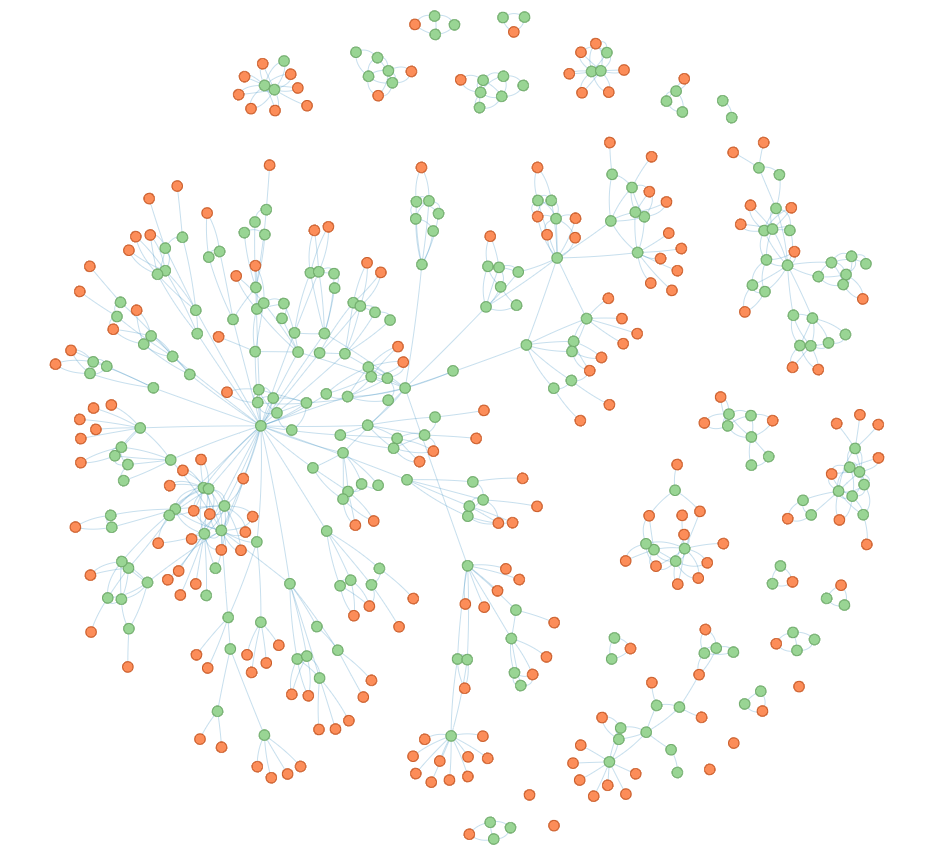
\includegraphics[width=1\linewidth]{/data/lfrancois/Development/DODO/inst/documentation/DODO-F1000-publication/fig/disNet_als_extension} 

}

\caption{The disNet build on the term 'amyotrophic lateral sclerosisr querying both labels and synonyms provided in DODO (green nodes). This disNet is subsequenctly extended to return all cross-reference identifiers and child terms using the extend\_disNet function (parameters 'relations = c('xref', 'child')' and to return only equivalent identifiers 'intransitive\_ambiguity = 1' is used (orange nodes).}\label{fig:disNetalsExtension}
\end{figure}

\textbf{CHEMBL}

There are 96 compounds identified through 4 identified (identifiers: MeSH:D000690, EFO:0000253, ORPHA:98756, EFO:0001356) using the disNet while 96 compounds identified through 3 disease identifiers (identifiers: MeSH:D000690, EFO:0000253, EFO:0001356.

Both approaches identify the same drug compounds but an additional disease was available through use of a disNet.

\begin{verbatim}
## 
##  EFO:0000253  EFO:0001356 MeSH:D000690  ORPHA:98756 
##           95            2           97            2
\end{verbatim}

\begin{verbatim}
## 
##  EFO:0000253  EFO:0001356 MeSH:D000690 
##           95            2           97
\end{verbatim}

This disease is a child term identified through extending the disNet (Figure \ref{fig:disnetALSchembl}). This term `ORPHA:98756' was identified as a child term of `EFO:0001356' with the extension of the disNet using DODO. The disease could not be identified through querying CHEMBL directly as it's labelled `Spinocerebellar ataxia type 2'". While this enriched extended network did not return additional compounds from CHEMBL in this example, the annotation of compounds used for treatment of ALS shows more granularity.

\begin{figure}

{\centering 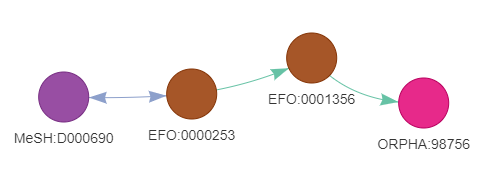
\includegraphics[width=0.5\linewidth]{/data/lfrancois/Development/DODO/inst/documentation/DODO-F1000-publication/fig/disNet_als_chembl} 

}

\caption{The visualized disNet shows the relations between the different diseases with compounds available in CHEMBL resource. This term 'ORPHA:98756' was identified as a child term of 'EFO:0001356' through extension (green edges). Cross-reference edge is\_xref are indicated in blue.  The disease could not be identified through querying CHEMBL directly as it's labelled 'Spinocerebellar ataxia type 2'. Using disease relationships present in DODO this node was identified additionally.}\label{fig:disnetALSchembl}
\end{figure}

\textbf{ClinVar}

All entrez gene identifiers identified by querying the ClinVar resource directly for ``amyotrophic lateral sclerosis'' were also returned when using the disNet disease network. Contrary, using the disNet build around ALS returns 1 additional Entrez gene identifiers reported for ClinVar identifier ClinVar:18286 with label: Inclusion body myopathy with early-onset Paget disease with or without frontotemporal dementia 2. This identifier was identified through extending through cross-references edges through transitivity mapping related to ``ORPHA:52430'' which carries ``Pagetoid amyotrophic lateral sclerosis'' as a synonym (Figure \ref{fig:disnetALSclinvar}).

\begin{figure}

{\centering 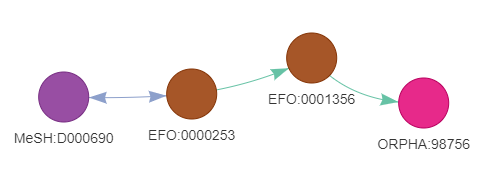
\includegraphics[width=0.5\linewidth]{/data/lfrancois/Development/DODO/inst/documentation/DODO-F1000-publication/fig/disNet_als_chembl} 

}

\caption{The visualized disNet shows how the identifier 'ClinVar:18286' ('Inclusion body myopathy with early-onset Paget disease with or without frontotemporal dementia 2') was returned through the use of transitivity on cross-reference edges starting from 'ORPHA:52430' ('Pagetoid amyotrophic lateral sclerosis'). With the is\_xref edges are indicated in blue and the is\_related edges indicated in orange.}\label{fig:disnetALSclinvar}
\end{figure}

\textbf{Tracing connections}

When obtaining a list of variants or compounds directly from the resources it isn't possible to understand if the return disease identiers that originate from different ontologies are always dealing with the same disease concepts. An additional feature from connecting resources through the use of a disNet, is the possibility to identify if and how diseases returned from each resource are connected to each other. This does not only allow a better understanding of disease, but also facilitates downstream analyses. Figure \ref{fig:traceConn} shows the original ALS disNet with disease identifiers matching in CHEMBL (orange) and those matching in ClinVar (blue). As both resources use different ontologies as references, there is a necessity to use cross-reference to understand their relationship to each other. Indirect relationships are used and recorded when extending and can facilitate the understanding and integration of different biological resources.

\begin{center}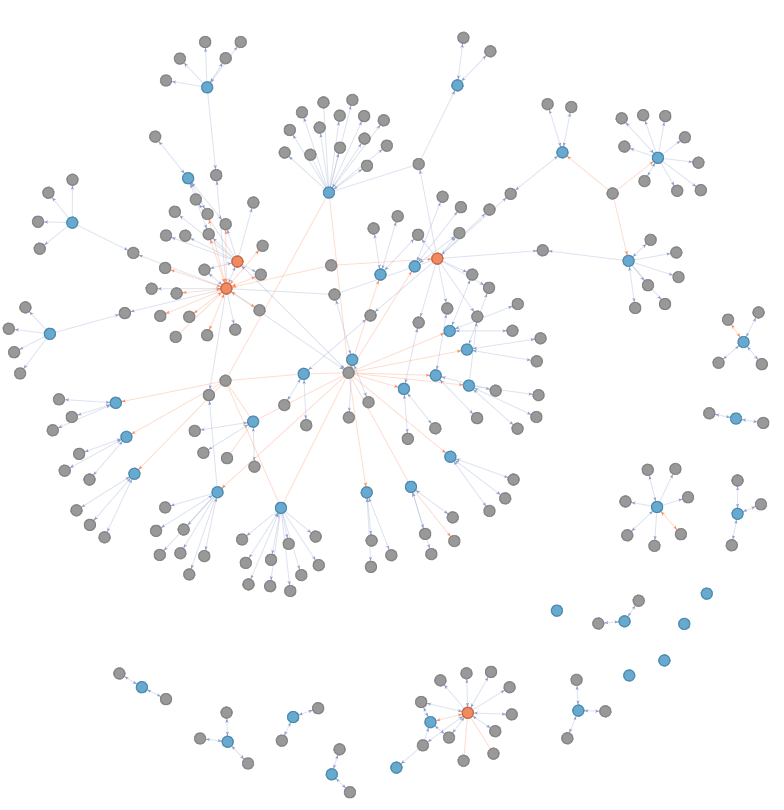
\includegraphics[width=1\linewidth]{/data/lfrancois/Development/DODO/inst/documentation/DODO-F1000-publication/fig/trace_connections} \end{center}

--\textgreater{}

\hypertarget{conclusions}{%
\section{Conclusions}\label{conclusions}}

Disease ontologies have allowed a more formal classification of diseases and could facilitate the integration of several biological databases to increase disease understanding and develop novel treatments. However, efforts to integrate biological databases or the ontologies directly are complicated by ontology-specific identifiers, heterogeneous decisions on disease definitions, and the inherent presence of errors. Despite this efforts, we identified two remaning challenges:

\begin{itemize}
\item
  Currently no resource provides a flexible and complete mapping across the multitude of disease ontologies
\item
  Availability of efficient and straightforward software on bioinformatics platform (R or python)
\end{itemize}

DODO R package contains several functions to build and interact with a disNet or convert concept identifiers between ontologies. The workflow to construct a custom, local DODO graphical database is provided with the intent to allow adaptation to specific needs and additional resources can be easily added without adaptation to the data model or R package.

We believe that DODO can help clarify and define conditions of interest and explore and visualize relationships between disease concepts. This allows the exploration of a disease and how correct the different mappings between ontologies are. This hopefully helps to increase disease understanding to people inside and outside of the medical field. In addition, connecting different biological database (information on compounds, text mining, transcriptomics, etc.) through a disNet ensures these resources are queried using different equivalent identifiers of the disease of interest without the user being required to make decisions on these mappings. In addition, it also allows visualizing the connection between these resources directly.

Through the aggregation of different ontologies and their mappings, DODO functions as a meta-database with easy access and possibility to estabblish a more exhaustive disease landscape. The code to build and query DODO is provided under open source license to allow further improvement by other developers.

--\textgreater{}

--\textgreater{}

\hypertarget{software-availability}{%
\section{Software availability}\label{software-availability}}

This section will be generated by the Editorial Office before publication. Authors are asked to provide some initial information to assist the Editorial Office, as detailed below.

\begin{enumerate}
\def\labelenumi{\arabic{enumi}.}
\item
  URL link to where the software can be downloaded from or used by a non-coder (AUTHOR TO PROVIDE; optional)
\item
  URL link to the author's version control system repository containing the source code (AUTHOR TO PROVIDE; required)
\item
  Link to source code as at time of publication (\emph{F1000Research} TO GENERATE)
\item
  Link to archived source code as at time of publication (\emph{F1000Research} TO GENERATE)
\item
  Software license (AUTHOR TO PROVIDE; required)
\end{enumerate}

\hypertarget{author-information}{%
\section{Author information}\label{author-information}}

In order to give appropriate credit to each author of an article, the individual contributions of each author to the manuscript should be detailed in this section. We recommend using author initials and then stating briefly how they contributed.

\hypertarget{competing-interests}{%
\section{Competing interests}\label{competing-interests}}

All financial, personal, or professional competing interests for any of the authors that could be construed to unduly influence the content of the article must be disclosed and will be displayed alongside the article. If there are no relevant competing interests to declare, please add the following: `No competing interests were disclosed'.

\hypertarget{grant-information}{%
\section{Grant information}\label{grant-information}}

Please state who funded the work discussed in this article, whether it is your employer, a grant funder etc. Please do not list funding that you have that is not relevant to this specific piece of research. For each funder, please state the funder's name, the grant number where applicable, and the individual to whom the grant was assigned. If your work was not funded by any grants, please include the line: `The author(s) declared that no grants were involved in supporting this work.'

\hypertarget{acknowledgments}{%
\section{Acknowledgments}\label{acknowledgments}}

This section should acknowledge anyone who contributed to the research or the article but who does not qualify as an author based on the criteria provided earlier (e.g.~someone or an organization that provided writing assistance). Please state how they contributed; authors should obtain permission to acknowledge from all those mentioned in the Acknowledgments section.

Please do not list grant funding in this section.

\hypertarget{additional-advice-to-authors}{%
\section{Additional advice to authors}\label{additional-advice-to-authors}}

The content above is either taken directly from the F1000Research \LaTeX~template, or has been adpated to suit R Markdown. Here we provide some additional advice to authors based on our own and other users' experiences of article submission to F1000Research, which will hopefully make your own journey smoother. If you would like to contribute to this, please contact us at \url{https://github.com/grimbough/BiocWorkflowTools/issues/4}

\begin{itemize}
\item
  When writing figure or tables captions do not use acronyms or abbreviations without explanation in the legend itself, even this has been addressed in the main text. F1000Research require each figure and table to be able to stand alone from the rest of the manuscript. \emph{Thanks to Mike Love \href{https://twitter.com/mikelove}{@mikelove}}
\end{itemize}

\bibliography{DODO.bib}

\end{document}
